\chapter{Assets and Architecture}
\begin{figure}[H]
\centering
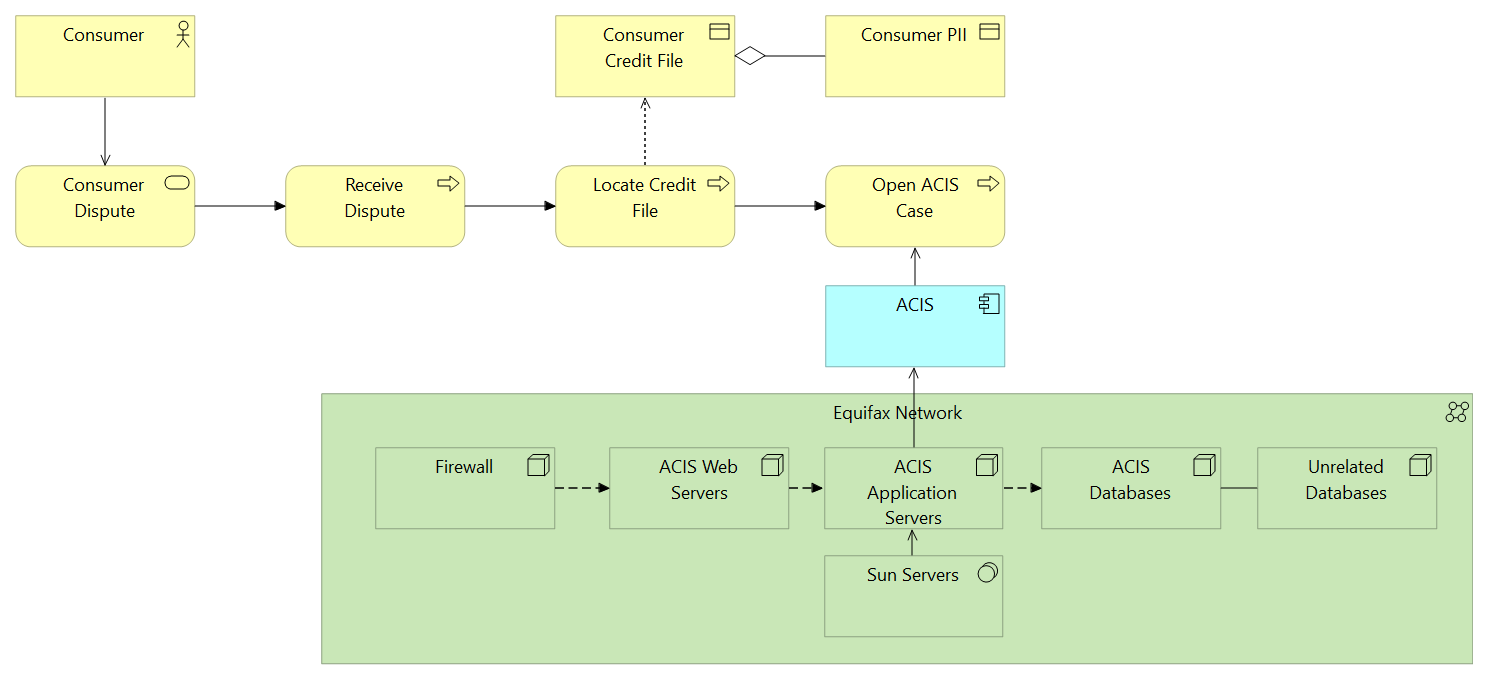
\includegraphics[width=1\linewidth]{images/asset-dependency-view.png}
\caption{Asset \& dependency view.}
\end{figure}

The given view identifies the main assets involved in the incident and shows how they are related to each other. 
\newline
The business layer provides an overview of the Equifax's consumer dispute process. Due to regulatory requirements, Equifax has to provide a way for consumers to dispute incorrect information on their consumer reports. One way for consumers to do it, is through an online process. When consumers file a dispute through their online service, Equifax receives their dispute, tracks their credit file containing their consumer information and lastly, opens an ACIS case to open an investigation on the dispute. 
\newline
This process depends on the ACIS application which makes up the application layer in the view.
\newline
ACIS itself it supported by it's web servers, application servers, databases and Sun servers withing the Equifax network. This infrastructure makes up the technology layer in this view and shows that the consumer dispute process ultimately relies on ACIS and it's underlying infrastructure.
\newline
Additionally, the technology layer also consists of databases unrelated to ACIS itself. This becomes important during the interview as these databases were accessed by the attackers during the incident as they were also in the same network as the ACIS environment.